\graphicspath{{./figures}}

% Project Planning
\chapter{Project Planning}
\textcolor{red}{Still to be formulated into a gantt chart}
Week 01 (24/07 to 30/07): Problem formulation; requirements gathering
Week 02 (31/07 to 06/08): Initial research; component selection
Week 03 (07/08 to 13/08): System-level design; initial system layout; components ordered
Week 04 (14/08 to 20/08): PCB design without traces; initial circuit design
Week 05 (21/08 to 27/08): Component prototyping; Full PCB design; initial antenna design;
Week 06 (28/08 to 03/09): Mechanical design; Custom link investigation; PCB ordered
Week 07 (04/09 to 10/09): (Test week)
Week 08 (11/09 to 17/09): Initial build
Week 09 (18/09 to 24/09): Software design; initial testing
Week 10 (25/09 to 01/10): Software design; debugging
Week 11 (02/10 to 08/10): Reporting
Week 12 (09/10 to 15/10): Design improvement
Week 13 (16/10 to 22/10): Testing
Week 14 (23/10 to 29/10): Reporting
Week 15 (30/10 to 05/11):

% Standards
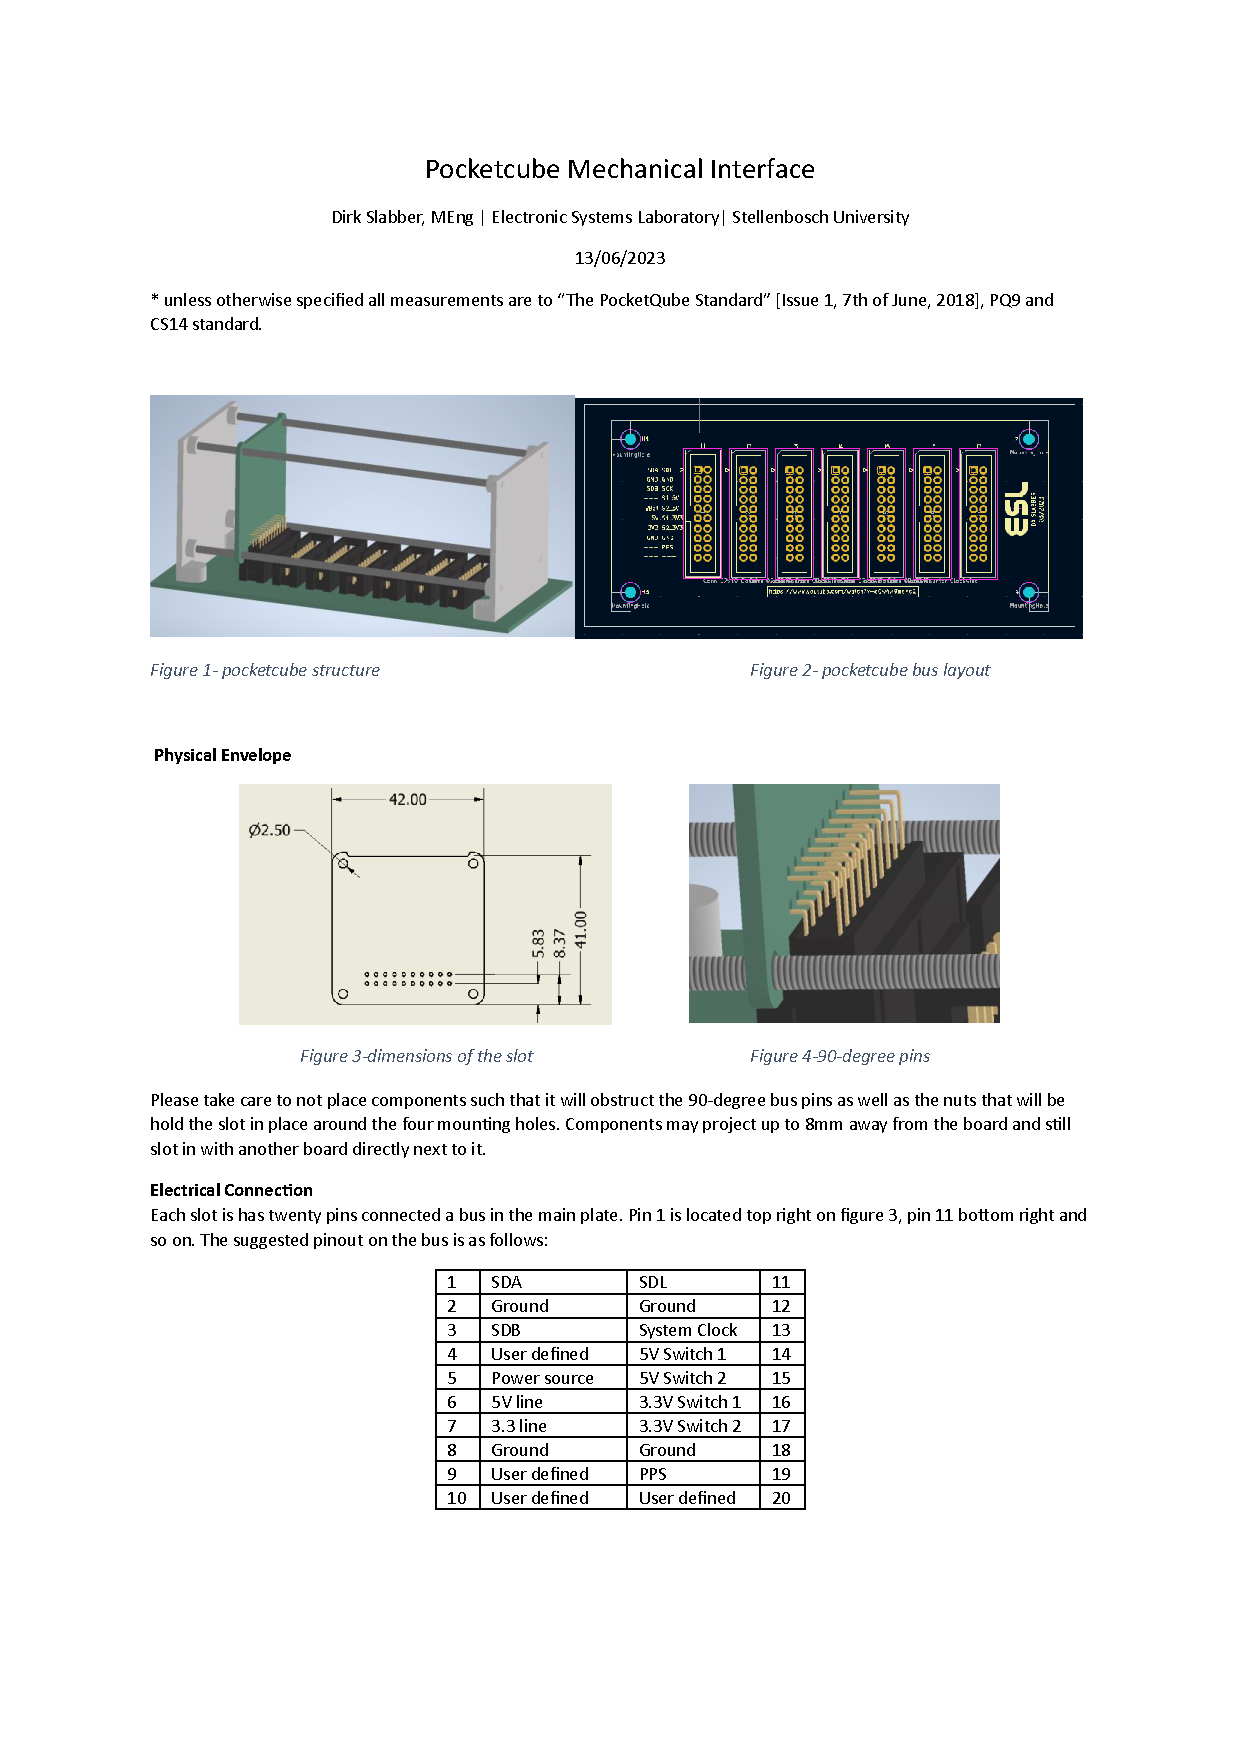
\includepdf[scale=0.8,pages=1,offset=0mm -35mm,pagecommand=\chapter{References}\section{PQSU}\label{sec:appendix_pqsu}]{docs/pqsu}
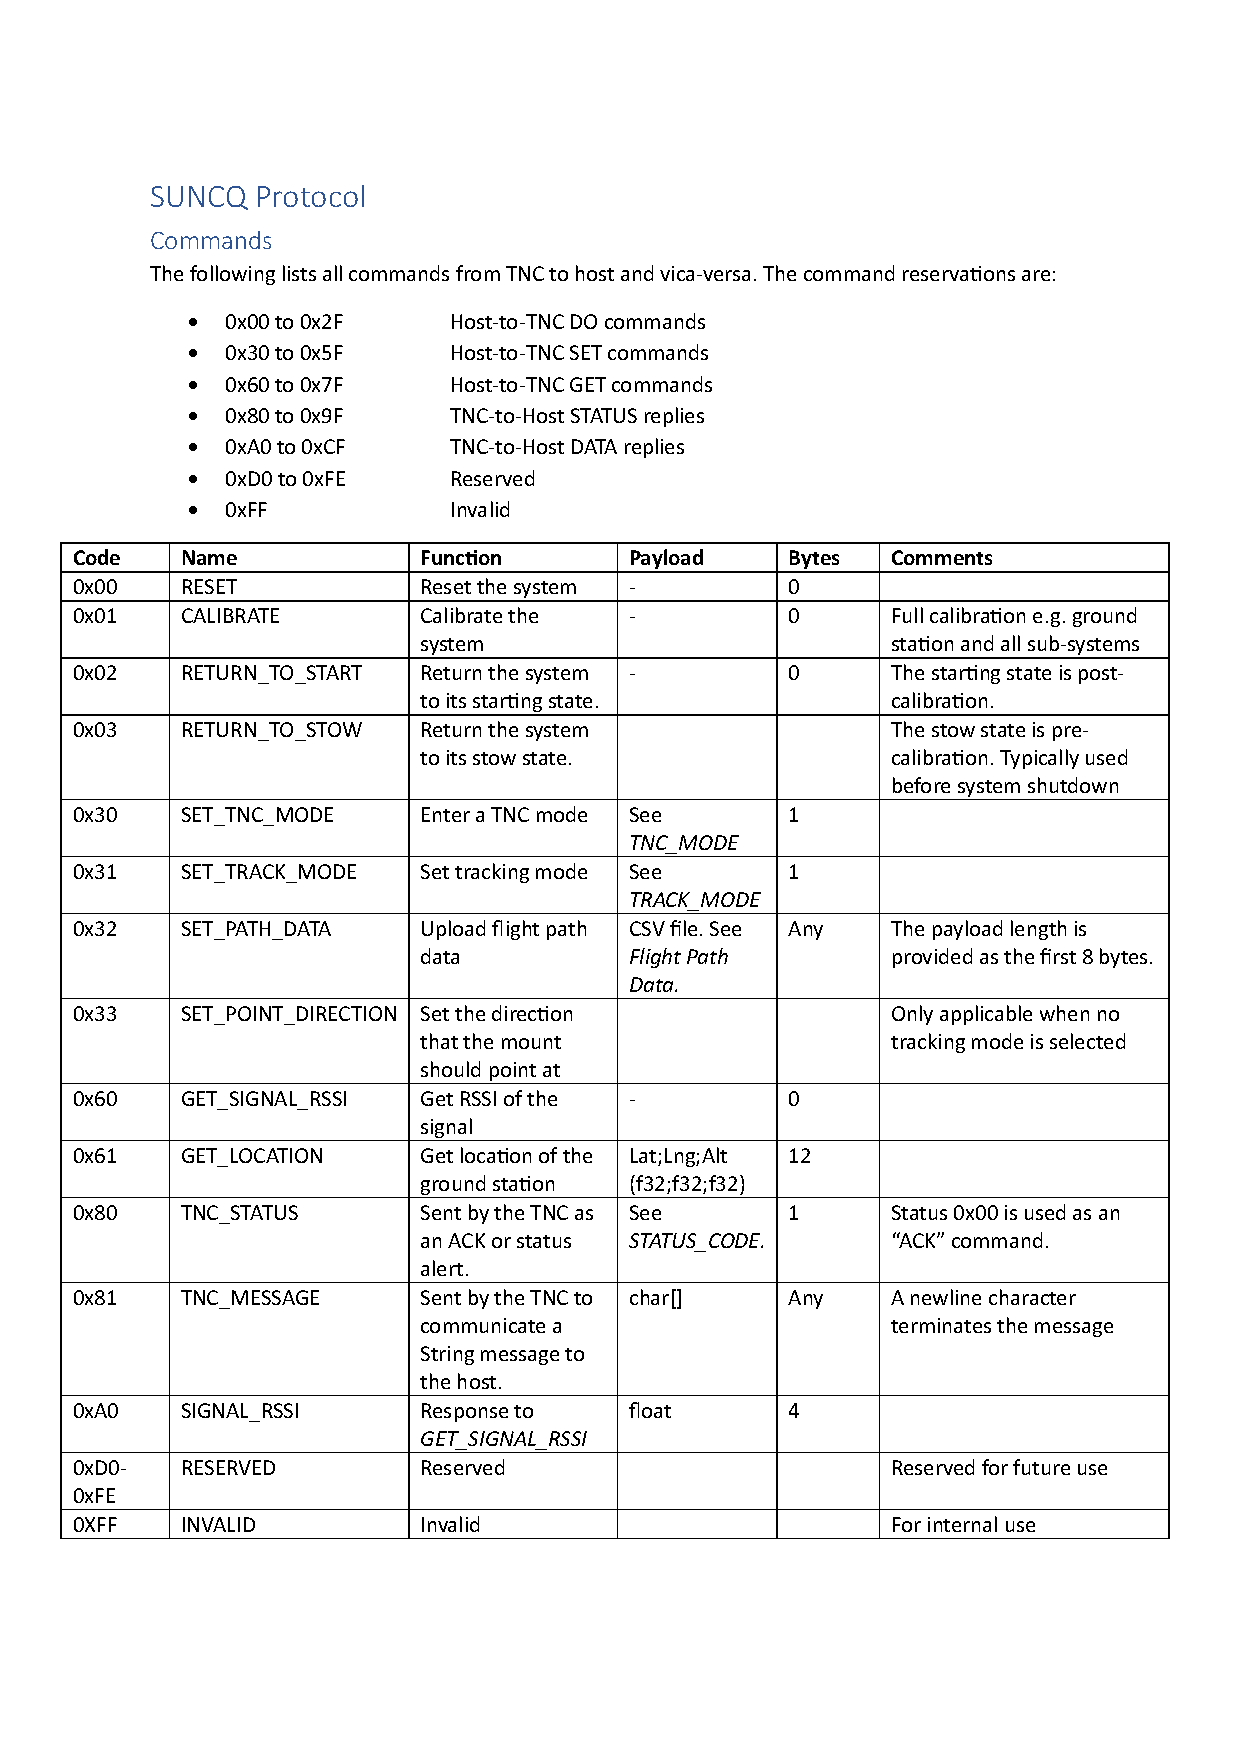
\includepdf[scale=0.85,pages=1,pagecommand=\section{SUNCQ}\label{sec:appendix_suncq}]{docs/suncq}
\includepdf[scale=0.85,pages=2]{docs/suncq}
\section{Antenna Gain}
\begin{figure}[!htb]
  \centering
  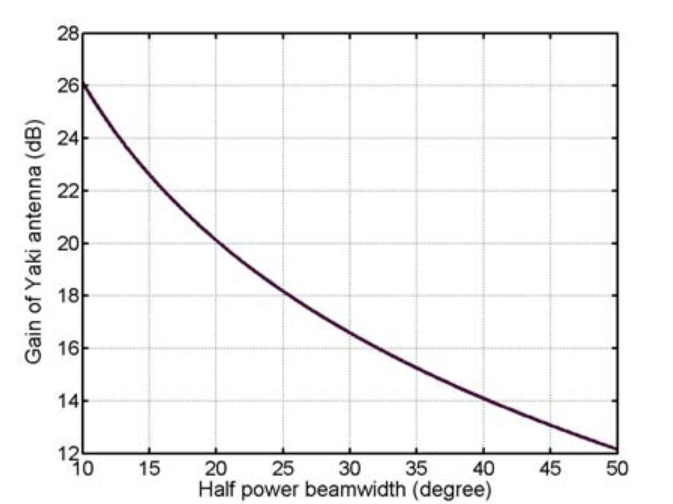
\includegraphics[width=0.5\textwidth]{antennaGain}
  \caption{Antenna Gain vs Beamwidth \cite{paper-yagiGainBeamwidth}}
  \label{fig:antennaGain}
\end{figure}

% Designs
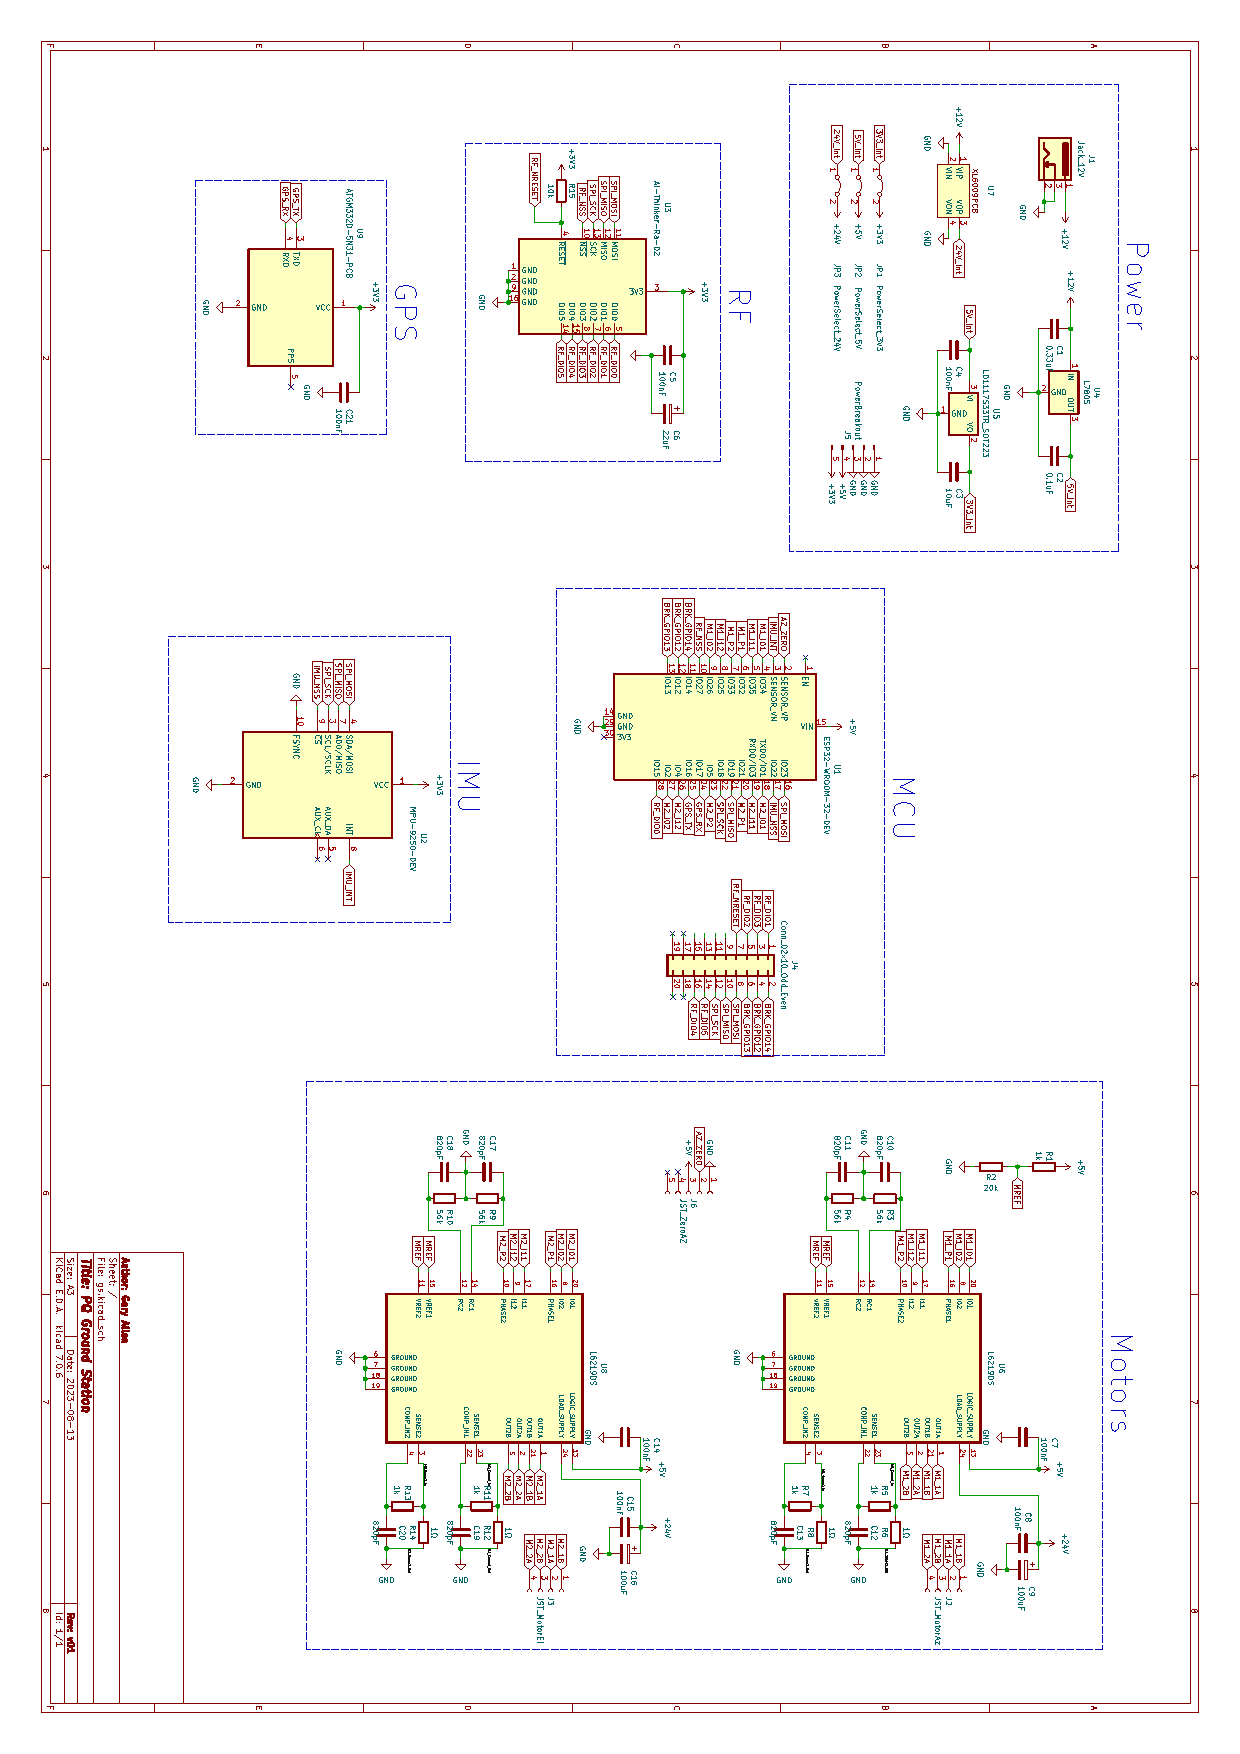
\includepdf[scale=0.65,pages=1,offset=0mm -35mm,pagecommand=\chapter{Design}\section{Ground Station Schematic}\label{sec:appendix_gs_schematics}]{docs/gs_schematic}
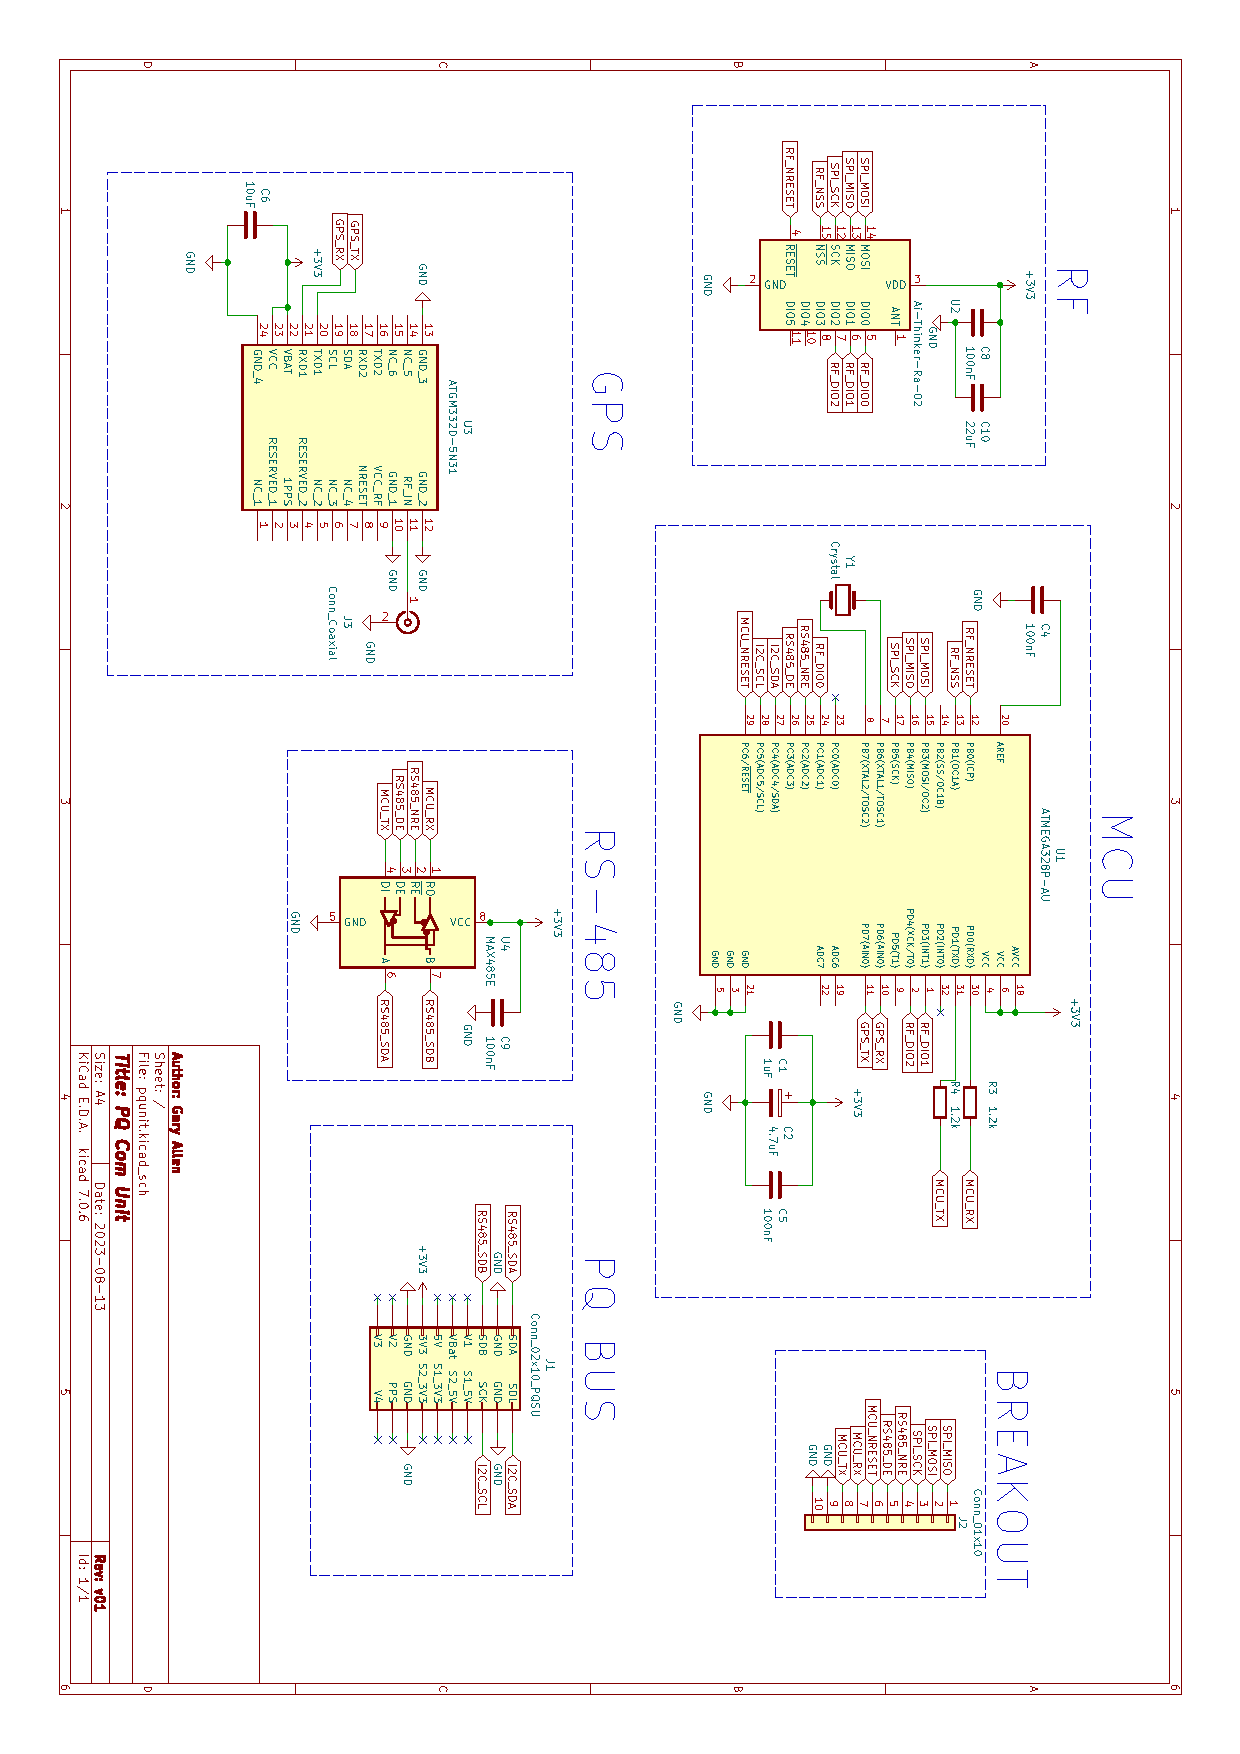
\includepdf[scale=0.7,pages=1,pagecommand=\section{PocketQube Unit Schematic}\label{sec:appendix_pq_schematic}]{docs/pq_schematic}
\section{Ground Station PCB}\label{sec:appendix_gs_pcb_design}
\begin{figure}[!htb]
  \centering
  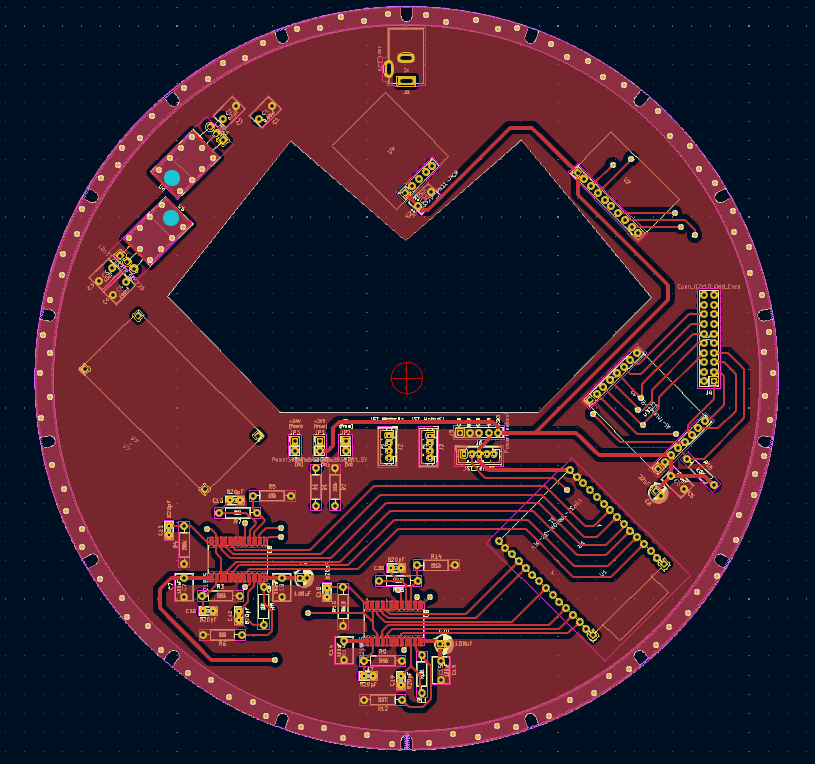
\includegraphics[width=0.6\textwidth]{gs_pcb_design}
  \caption{Ground Station PCB Design}
  \label{fig:gs_pcb}
\end{figure}
\section{PCB Errata}\label{sec:appendix_pcb_errata}
\begin{itemize}
    \item \textcolor{red}{Full errata for PCB designs still to be added}
\end{itemize}
\section{Software}
\begin{table}[!htb]
  \centering
  \caption{GPS Class}
  \renewcommand{\arraystretch}{1.2}
  \begin{tabular}{ |c|c| }
  \hline
  \textbf{Function}        & \textbf{Description}    \\
  \hline
    getLocation()              & Return latitude, longitude and altitude \\
    getTime()                  & Return seconds since epoch \\
  \hline
  \end{tabular}
  \label{tab:gpsUML}
\end{table}

\begin{table}[!htb]
  \centering
  \caption{Radio Class}
  \renewcommand{\arraystretch}{1.2}
  \begin{tabular}{ |c|c| }
  \hline
  \textbf{Function}        & \textbf{Description}    \\
  \hline
    startTransmit(message)              & Transmit data (non-blocking i.e. with callback) \\
    startReceive()                      & Start listening to receive data (non-blocking i.e. with callback) \\
    getRssi()                           & Get signal strength \\
    getSnr()                            & Get signal-to-noise ratio \\
  \hline
  \end{tabular}
  \label{tab:radioUML}
\end{table}

\begin{table}[!htb]
  \centering
  \caption{Link Class}
  \renewcommand{\arraystretch}{1.2}
  \begin{tabular}{ |c|c| }
  \hline
  \textbf{Function}        & \textbf{Description}    \\
  \hline
  setTelemetryCallback(fn)                    & Set the "telemetry sent/received" function  \\
  setTelecommandCallback(fn)                  & Set the "telecommand received" function (\textit{Responder} only) \\
  \hline
  \end{tabular}
  \label{tab:linkUML}
\end{table}

\begin{table}[!htb]
  \centering
  \caption{StepperMotor Class}
  \renewcommand{\arraystretch}{1.2}
  \begin{tabular}{ |c|c| }
  \hline
  \textbf{Function}        & \textbf{Description}    \\
  \hline
    stepForward(numSteps)         & Blocking and non-blocking options \\
    saveZeroPosition()            & Used for calibration \\
    getPosition()                 & Used for open-loop feedback \\
    setSpeed()                    & Sets the delay between steps \\
    setCurrentMultiplier()        & Set the amount of current \\
  \hline
  \end{tabular}
  \label{tab:stepperMotorUML}
\end{table}

\begin{table}[!htb]
  \centering
  \caption{Mount Class}
  \renewcommand{\arraystretch}{1.2}
  \begin{tabular}{ |c|c| }
  \hline
  \textbf{Function}        & \textbf{Description}    \\
  \hline
    calibrate()                         & Calbrate the mount \\
    setAzimuthalElevation(az, el)       & Set the azimuthal and elevation angles \\
    setBoresight(boresightVec)          & Set the boresight pointing vector \\
  \hline
  \end{tabular}
  \label{tab:mountUML}
\end{table}

\begin{table}[!htb]
  \centering
  \caption{GroundStation Class}
  \renewcommand{\arraystretch}{1.2}
  \begin{tabular}{ |c|c| }
  \hline
  \textbf{Function}             & \textbf{Description}    \\
  \hline
    calibrate()                 & Calibrate the entire GS \\
    addEstimatedLocation(loc)      & Add an estimated input GPS location for open-loop tracking \\
    addKnownLocation(loc)          & Add a known GPS location for closed-loop tracking \\
  \hline
  \end{tabular}
  \label{tab:groundStationUML}
\end{table}


% Hardware
\chapter{Hardware}
\section{Existing Mount PCB}\label{sec:appendix_gs_pcb_existing}
\begin{figure}[!htb]
  \centering
  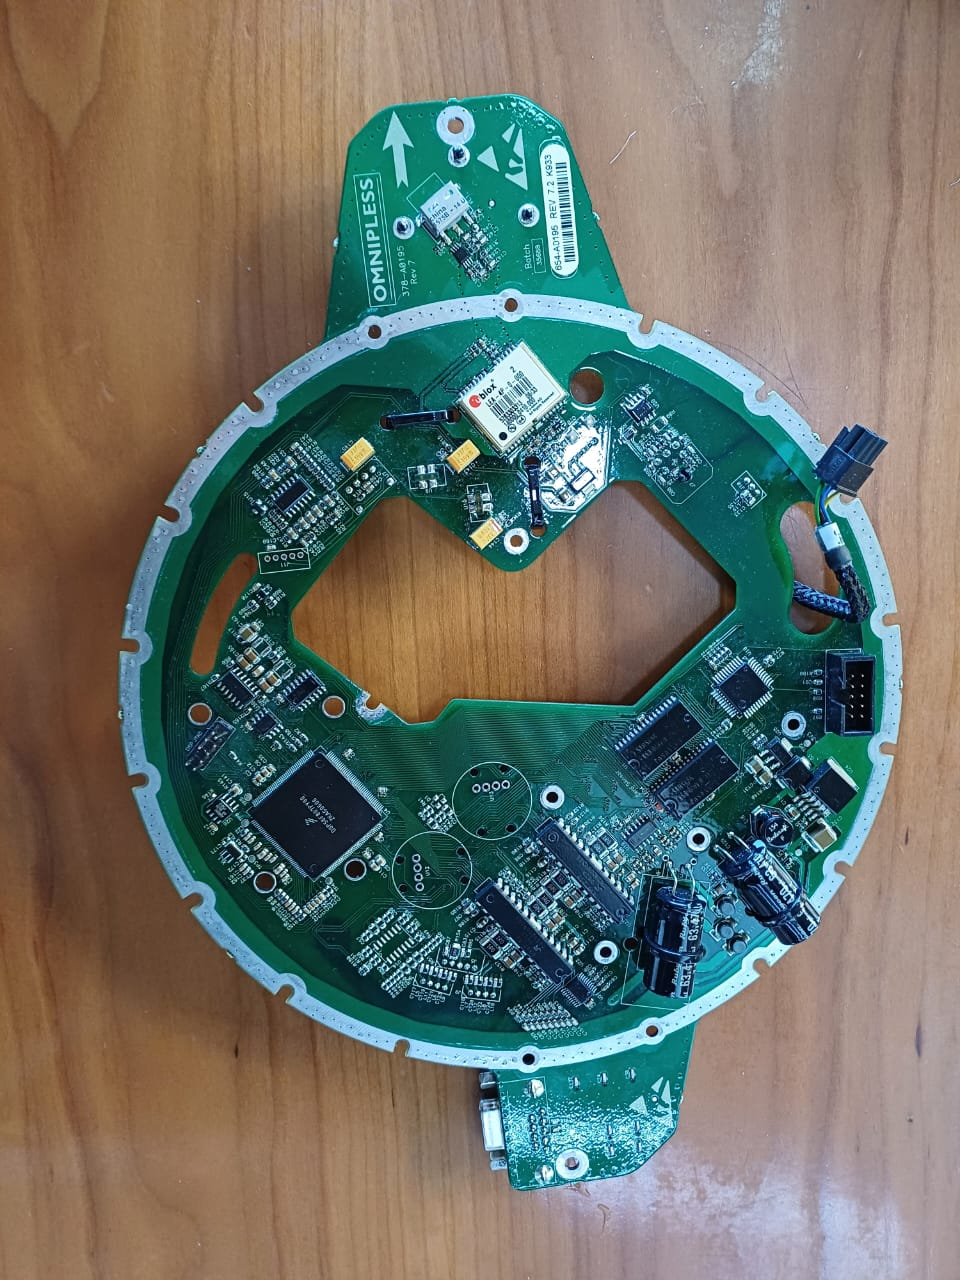
\includegraphics[width=0.4\textwidth, angle=90, origin=c]{gs_existing}
  \caption{Existing Antenna Mount PCB}
  \label{fig:gs_existing}
\end{figure}
\newpage
\section{PocketQube}\label{sec:appendix_pq}
\begin{figure}[!htb]
    \centering
    \includegraphics[width=0.7\textwidth]{pqBreadboard}
    \caption{PocketQube Breadboard for Testing}
    \label{fig:pqBreadboard}
\end{figure}
\begin{figure}[!htb]
  \centering
  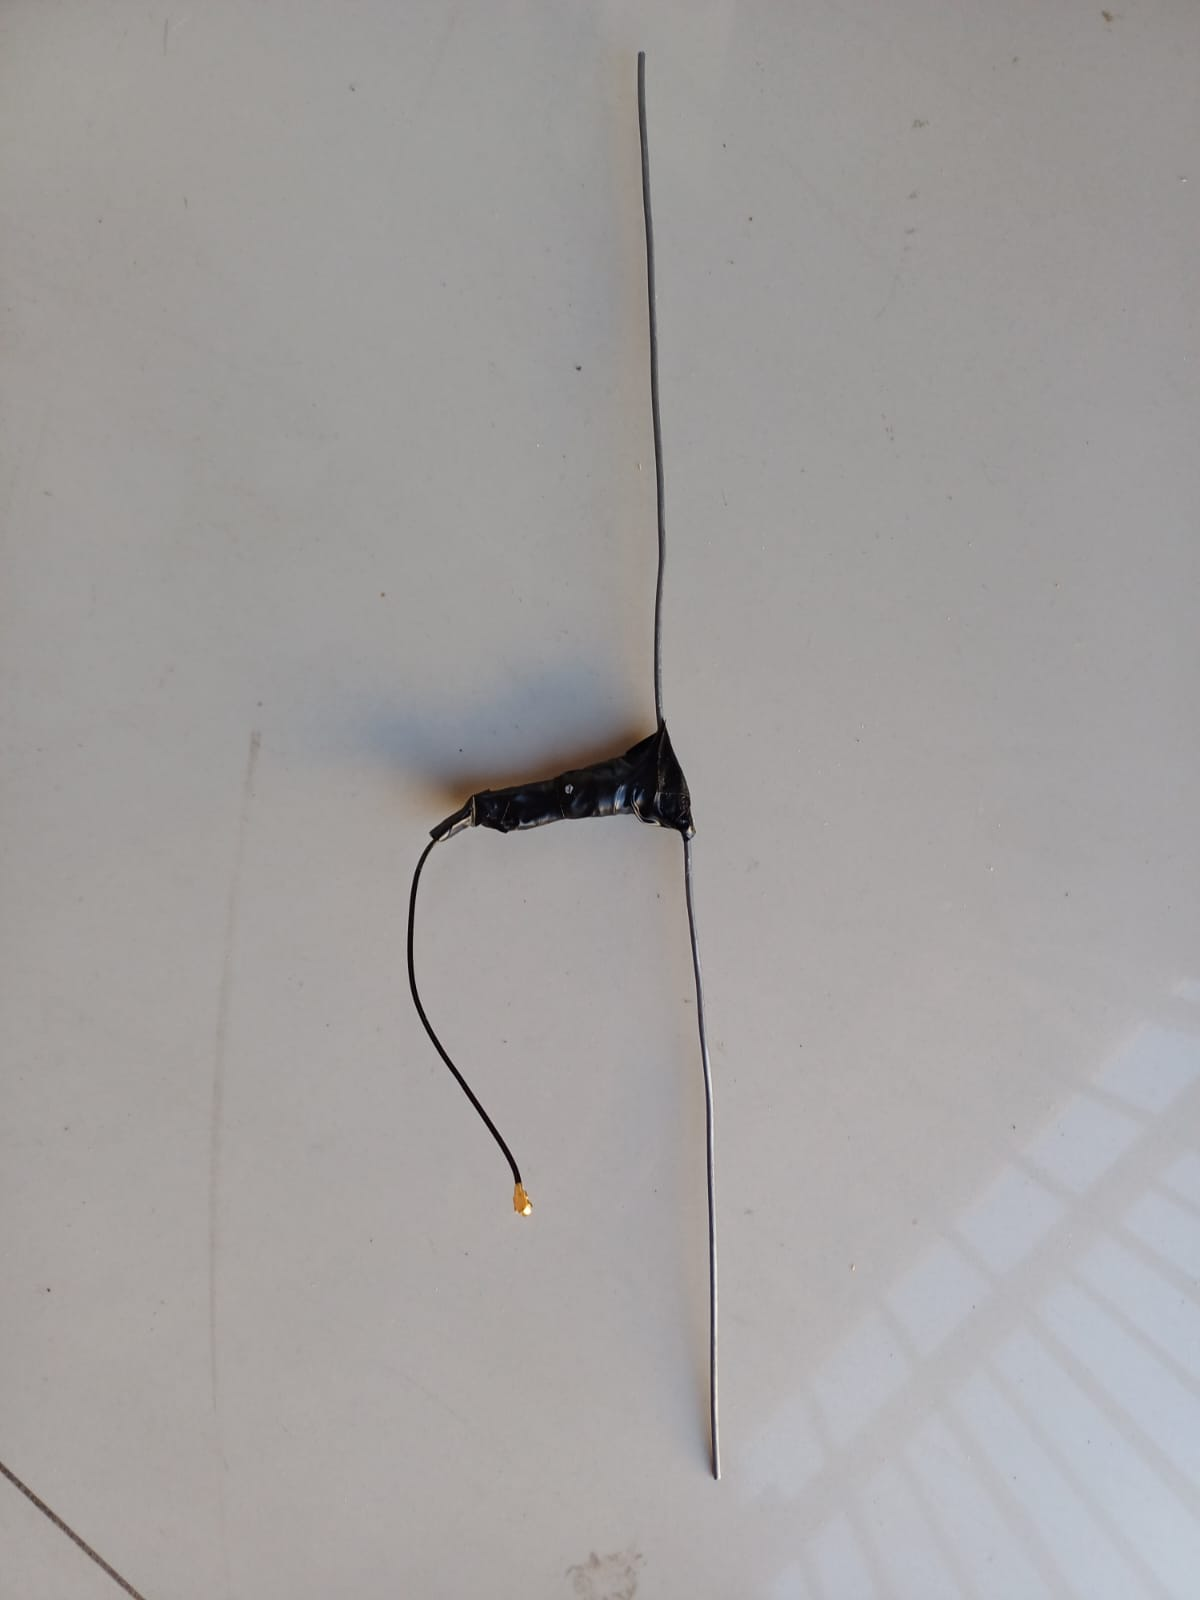
\includegraphics[width=0.5\textwidth,angle=90]{pqAntenna}
  \caption{PocketQube Dipole Antenna}
  \label{fig:pqAntenna}
\end{figure}
\newpage
\section{Mount Rotation}\label{sec:appendix_mount_rotation}
\begin{figure}[!htb]
  \begin{minipage}{.32\textwidth}
    \centering
    \includegraphics[width=0.95\linewidth,angle=270]{mountRotation1}
    \caption{Mount Azimuthal Compensation 1 (Elevation Fixed)}
    \label{fig:mountCompensation1}
  \end{minipage}
  \begin{minipage}{.32\textwidth}
    \centering
    \includegraphics[width=0.95\linewidth,angle=270]{mountRotation2}
    \caption{Mount Azimuthal Compensation 2 (Elevation Fixed)}
    \label{fig:mountCompensation2}
  \end{minipage}
  \begin{minipage}{.32\textwidth}
    \centering
    \includegraphics[width=0.95\linewidth,angle=270]{mountRotation3}
    \caption{Mount Azimuthal Compensation 3 (Elevation Fixed)}
    \label{fig:mountCompensation3}
  \end{minipage}
\end{figure}
\begin{figure}[!htb]
  \begin{minipage}{.32\textwidth}
    \centering
    \includegraphics[width=0.95\linewidth,angle=270]{mountRotation4}
    \caption{Mount Azimuthal Compensation 4 (Elevation Fixed)}
    \label{fig:mountCompensation4}
  \end{minipage}
  \begin{minipage}{.32\textwidth}
    \centering
    \includegraphics[width=0.95\linewidth,angle=270]{mountRotation6}
    \caption{Mount Azimuthal Compensation 5 (Azimuth Fixed)}
    \label{fig:mountCompensation5}
  \end{minipage}
  \begin{minipage}{.32\textwidth}
    \centering
    \includegraphics[width=0.95\linewidth,angle=270]{mountRotation7}
    \caption{Mount Azimuthal Compensation 6 (Azimuth Fixed)}
    \label{fig:mountCompensation6}
  \end{minipage}
\end{figure}

% Software
\chapter{Software}
\section{GUI}\label{sec:appendix_gui}
\begin{figure}[!htb]
  \centering
  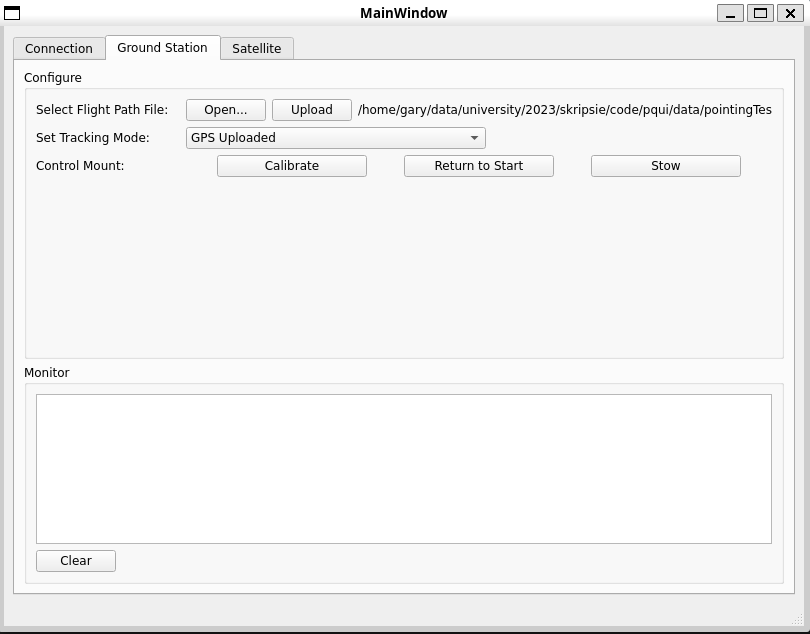
\includegraphics[width=0.95\textwidth]{guiSnapshot1}
  \caption{GUI Snapshot}
  \label{fig:guiSnapshot}
\end{figure}

% Tests
\chapter{Tests}
\section{Range Tests}\label{sec:appendix_range}
\begin{figure}[!htb]
  \centering
  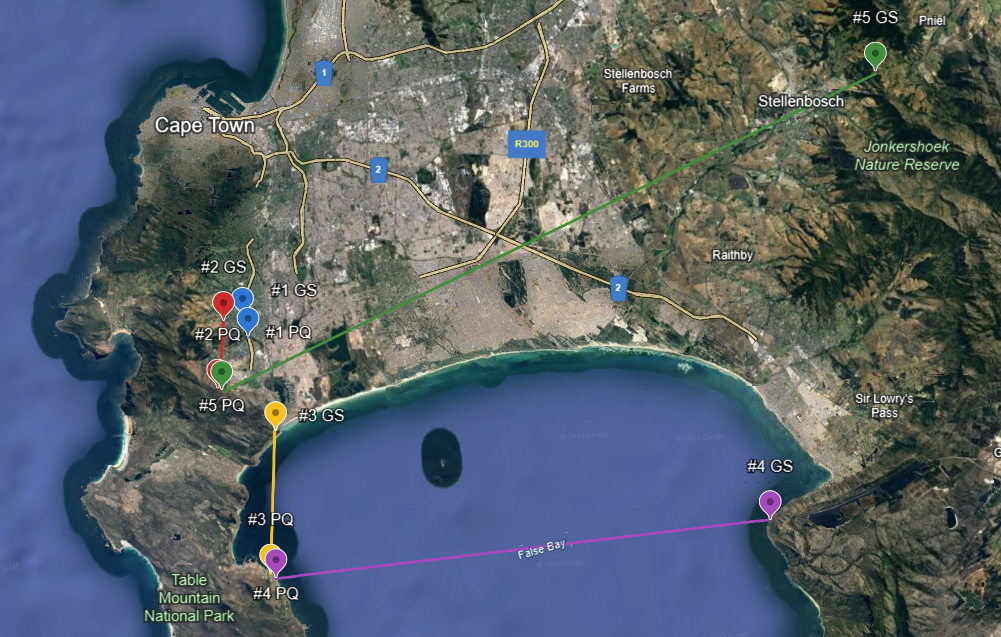
\includegraphics[width=0.8\textwidth]{rangeTests}
  \caption{Range Test Locations}
  \label{fig:rangeTests}
\end{figure}